\clearpage
\subsection{Understanding RNN, LSTM, and GRU}
\label{app:rnn}

\begin{figure}[H]
    \centering
    \caption{Comparison of RNN, LSTM, and GRU architectures,}
    \label{fig:rnn-lstm-gru}
    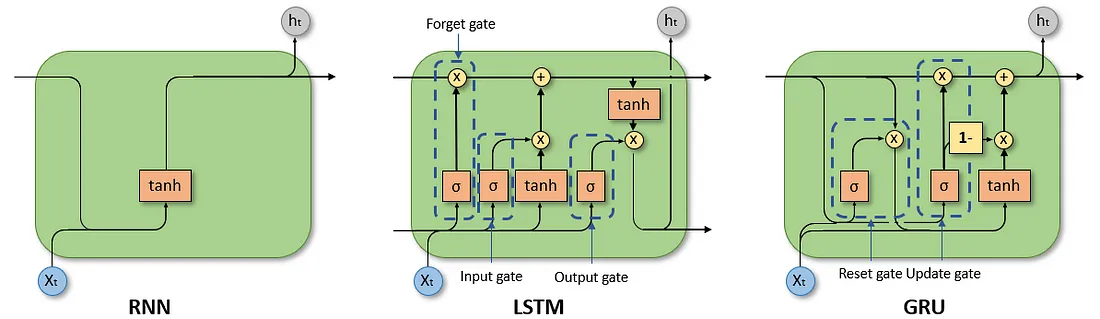
\includegraphics[width=\textwidth]{img/sections/back/rnn-lstm-gru.png}
\end{figure}

\acrfullpl{rnn} are a class of neural networks designed for sequential data processing. Unlike feedforward 
networks, \acrshortpl{rnn} incorporate loops that allow information to persist across time steps, making them well-suited 
for tasks involving sequential dependencies, such as natural language processing and time-series forecasting.

\paragraph{Architecture of RNN} An \acrshort{rnn} processes input sequences one element at a time while maintaining a
\emph{hidden state} that captures information about previous time steps. The recurrent nature of \acrshortpl{rnn} is 
represented mathematically as follows (Equation~\ref{eq:rnn_eq}):

\begin{equation}
    \label{eq:rnn_eq}
    h_t = \sigma(W_h h_{t-1} + W_x x_t + b)
\end{equation}

where:
\begin{itemize}
    \item $h_t$ is the hidden state at time step $t$
    \item $x_t$ is the input at time step $t$
    \item $W_h$ and $W_x$ are weight matrices
    \item $b$ is the bias term
    \item $\sigma$ is the activation function (commonly tanh or ReLU)
\end{itemize}

This architecture allows information to flow from past time steps to future ones~\parencite{nabipour2020DeepLearning}.

\paragraph{Limitations of RNNs}
One of the major issues with RNNs is the \emph{vanishing gradient problem}, which arises during \acrfull{bptt}. 
The gradients of earlier time steps shrink exponentially, making it difficult for the model to retain long-term 
dependencies~\parencite{parmar2018stock}.

\paragraph{LSTM Architecture} \acrfullpl{lstm} are a special type of \acrshort{rnn} designed to address the 
\emph{vanishing gradient problem}. They achieve this by introducing a \emph{memory cell} that can maintain 
information for long durations \parencite{phuoc2024StockPrediction}.

An \acrshort{lstm} unit consists of (Diagram in Figure~\ref{fig:rnn-lstm-gru}):
\begin{itemize}
\item \textbf{Forget Gate ($f_t$)} - Decides what part of the previous memory to retain.
\item \textbf{Input Gate ($i_t$)} - Regulates new information stored in the cell.
\item \textbf{Cell State ($C_t$)} - Represents the internal memory.
\item \textbf{Output Gate ($o_t$)} - Determines what information is sent to the next time step.
\end{itemize}

The computations for an \acrshort{lstm} cell are as follows:

\begin{align}
f_t &= \sigma(W_f [h_{t-1}, x_t] + b_f) \\
i_t &= \sigma(W_i [h_{t-1}, x_t] + b_i) \\
\tilde{C}t &= \tanh(W_C [h{t-1}, x_t] + b_C) \\
C_t &= f_t * C_{t-1} + i_t * \tilde{C}t \\
o_t &= \sigma(W_o [h{t-1}, x_t] + b_o) \\
h_t &= o_t * \tanh(C_t)
\end{align}

\paragraph{GRU Architecture} \acrfullpl{gru} simplify the architecture of \acrshortpl{lstm} by using only two 
gates~\parencite{chang2024StockPrediction}.

A \acrshort{gru} unit consists of:
\begin{itemize}
\item \textbf{Reset Gate ($r_t$)} - Controls how much past information should be forgotten.
\item \textbf{Update Gate ($z_t$)} - Determines the amount of new memory to retain versus past memory.
\end{itemize}

The computations for a \acrshort{gru} cell are as follows:

\begin{align}
r_t &= \sigma(W_r [h_{t-1}, x_t] + b_r) \\
z_t &= \sigma(W_z [h_{t-1}, x_t] + b_z) \\
\tilde{h}t &= \tanh(W_h [r_t * h{t-1}, x_t] + b_h) \\
h_t &= (1 - z_t) * h_{t-1} + z_t * \tilde{h}_t
\end{align}

\subsubsection{Understanding BiGRU}

\begin{figure}[H]
    \centering
    \caption{Structure of Bidirectional GRU (BiGRU): (a) GRU cell and (b) unroll BiGRU}
    \label{fig:bigru}
    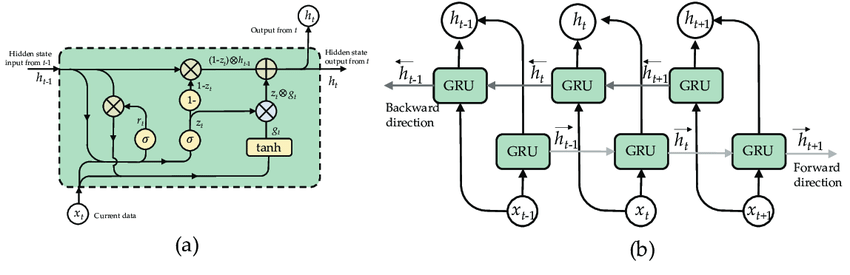
\includegraphics[width=\textwidth]{img/sections/back/bigru.png}
\end{figure}

\paragraph{BiGRU Architecture} \acrfull{bigru} is an extension of the standard \acrshort{gru} that improves sequence 
modeling by processing the input \emph{in both forward and backward directions}. This allows the network to capture 
\emph{context from both past and future time steps}, making it especially useful for tasks involving 
long-range dependencies~\parencite{shaban2024SMPDL}.

A \acrshort{bigru} processes information in two directions:
\begin{align}
\overrightarrow{h_t} &= \text{GRU}(x_t, \overrightarrow{h_{t-1}}) \\
\overleftarrow{h_t} &= \text{GRU}(x_t, \overleftarrow{h_{t+1}}) \\
h_t^{\text{BiGRU}} &= [\overrightarrow{h_t}; \overleftarrow{h_t}]
\end{align}

where:
\begin{itemize}
\item $\overrightarrow{h_t}$ is the forward GRU output.
\item $\overleftarrow{h_t}$ is the backward GRU output.
\end{itemize}

\paragraph{Advantages of BiGRU Over GRU}

\begin{itemize}
\item \emph{Captures both past and future context} at each time step.
\item \emph{Improved performance} in time-series forecasting.
\end{itemize}

\subsubsection{Understanding Hybrid Models: LSTM-GRU and LSTM-BiGRU}

Hybrid models like \acrshort{lstmgru} and \acrshort{lstmbigru} are used to leverage the strengths of
different architectures and improve the 
accuracy, efficiency, and generalization of deep learning models in sequence-based tasks. \acrshort{lstm} is excellent at 
capturing long-term dependencies due to its gating mechanisms, which prevent vanishing gradients. However, \acrshort{gru} 
is computationally more efficient and requires fewer parameters, making it a faster alternative with comparable 
performance~\parencite{phuoc2024StockPrediction}. Combining LSTM and GRU allows models to balance memory retention and computational
efficiency, effectively capturing both short-term and long-term dependencies.

